% Options for packages loaded elsewhere
% Options for packages loaded elsewhere
\PassOptionsToPackage{unicode}{hyperref}
\PassOptionsToPackage{hyphens}{url}
%
\documentclass[
  ignorenonframetext,
  aspectratio=169,
  russian,
]{beamer}
\newif\ifbibliography
\usepackage{pgfpages}
\setbeamertemplate{caption}[numbered]
\setbeamertemplate{caption label separator}{: }
\setbeamercolor{caption name}{fg=normal text.fg}
\beamertemplatenavigationsymbolshorizontal
% remove section numbering
\setbeamertemplate{part page}{
  \centering
  \begin{beamercolorbox}[sep=16pt,center]{part title}
    \usebeamerfont{part title}\insertpart\par
  \end{beamercolorbox}
}
\setbeamertemplate{section page}{
  \centering
  \begin{beamercolorbox}[sep=12pt,center]{section title}
    \usebeamerfont{section title}\insertsection\par
  \end{beamercolorbox}
}
\setbeamertemplate{subsection page}{
  \centering
  \begin{beamercolorbox}[sep=8pt,center]{subsection title}
    \usebeamerfont{subsection title}\insertsubsection\par
  \end{beamercolorbox}
}
% Prevent slide breaks in the middle of a paragraph
\widowpenalties 1 10000
\raggedbottom
\AtBeginPart{
  \frame{\partpage}
}
\AtBeginSection{
  \ifbibliography
  \else
    \frame{\sectionpage}
  \fi
}
\AtBeginSubsection{
  \frame{\subsectionpage}
}
\usepackage{iftex}
\ifPDFTeX
  \usepackage[T1]{fontenc}
  \usepackage[utf8]{inputenc}
  \usepackage{textcomp} % provide euro and other symbols
\else % if luatex or xetex
  \usepackage{unicode-math} % this also loads fontspec
  \defaultfontfeatures{Scale=MatchLowercase}
  \defaultfontfeatures[\rmfamily]{Ligatures=TeX,Scale=1}
\fi
\usepackage{lmodern}

\ifPDFTeX\else
  % xetex/luatex font selection
\fi
% Use upquote if available, for straight quotes in verbatim environments
\IfFileExists{upquote.sty}{\usepackage{upquote}}{}
\IfFileExists{microtype.sty}{% use microtype if available
  \usepackage[]{microtype}
  \UseMicrotypeSet[protrusion]{basicmath} % disable protrusion for tt fonts
}{}


\usepackage{longtable,booktabs,array}
\newcounter{none} % for unnumbered tables
\usepackage{calc} % for calculating minipage widths
\usepackage{caption}
% Make caption package work with longtable
\makeatletter
\def\fnum@table{\tablename~\thetable}
\makeatother
\usepackage{graphicx}
\makeatletter
\newsavebox\pandoc@box
\newcommand*\pandocbounded[1]{% scales image to fit in text height/width
  \sbox\pandoc@box{#1}%
  \Gscale@div\@tempa{\textheight}{\dimexpr\ht\pandoc@box+\dp\pandoc@box\relax}%
  \Gscale@div\@tempb{\linewidth}{\wd\pandoc@box}%
  \ifdim\@tempb\p@<\@tempa\p@\let\@tempa\@tempb\fi% select the smaller of both
  \ifdim\@tempa\p@<\p@\scalebox{\@tempa}{\usebox\pandoc@box}%
  \else\usebox{\pandoc@box}%
  \fi%
}
% Set default figure placement to htbp
\def\fps@figure{htbp}
\makeatother



\ifLuaTeX
\usepackage[bidi=basic,shorthands=off,provide=*]{babel}
\else
\usepackage[bidi=default,shorthands=off,provide=*]{babel}
\fi
\ifLuaTeX
  \usepackage{selnolig} % disable illegal ligatures
\fi


\setlength{\emergencystretch}{3em} % prevent overfull lines

\providecommand{\tightlist}{%
  \setlength{\itemsep}{0pt}\setlength{\parskip}{0pt}}



 

\usepackage[]{csquotes}

%%% Load theme
\IfFileExists{beamerthemegotham.sty}{
  %%%% Full TeXlive
  \usetheme{gotham}
  \gothamset{
    numbering=totalframenumber,
    parttocframe default=off,
    sectiontocframe default=off,
    subsectiontocframe default=off,
    tocframe template=gotham bullet,
    progressbar position=foot,
  }
  
  % 把背景画布清空（干掉那个巨大的地球）
  \setbeamertemplate{background canvas}{}
  
  \renewcommand{\gothamInstituteLogoSquare}[1][4ex]{%
    
\includegraphics[height=##1]{_resources/image/logo_rudn-inverted.png}
  }
}{%
  %%%% TinyTeX
  \usepackage{libertine}
  \usetheme{Madrid}
}
\makeatletter
\@ifpackageloaded{caption}{}{\usepackage{caption}}
\AtBeginDocument{%
\ifdefined\contentsname
  \renewcommand*\contentsname{Содержание}
\else
  \newcommand\contentsname{Содержание}
\fi
\ifdefined\listfigurename
  \renewcommand*\listfigurename{Список иллюстраций}
\else
  \newcommand\listfigurename{Список иллюстраций}
\fi
\ifdefined\listtablename
  \renewcommand*\listtablename{Список таблиц}
\else
  \newcommand\listtablename{Список таблиц}
\fi
\ifdefined\figurename
  \renewcommand*\figurename{Рисунок}
\else
  \newcommand\figurename{Рисунок}
\fi
\ifdefined\tablename
  \renewcommand*\tablename{Таблица}
\else
  \newcommand\tablename{Таблица}
\fi
}
\@ifpackageloaded{float}{}{\usepackage{float}}
\floatstyle{ruled}
\@ifundefined{c@chapter}{\newfloat{codelisting}{h}{lop}}{\newfloat{codelisting}{h}{lop}[chapter]}
\floatname{codelisting}{Список}
\newcommand*\listoflistings{\listof{codelisting}{Листинги}}
\makeatother
\makeatletter
\makeatother
\makeatletter
\@ifpackageloaded{caption}{}{\usepackage{caption}}
\@ifpackageloaded{subcaption}{}{\usepackage{subcaption}}
\makeatother

\usepackage{bookmark}
\IfFileExists{xurl.sty}{\usepackage{xurl}}{} % add URL line breaks if available
\urlstyle{same}
% fallback for those not using the hyperref driver hyperxmp:
\makeatletter
\@ifundefined{xmpquote}{\newcommand{\xmpquote}[1]{#1}}{}
\makeatother
\hypersetup{
  pdftitle={Лабораторная работа № 1},
  pdfauthor={Чжао Синья},
  pdflang={ru},
  hidelinks,
  pdfcreator={LaTeX via pandoc}}


\title{\texorpdfstring{Лабораторная работа №
1}{Лабораторная работа № 1}}
\subtitle{\texorpdfstring{Установка и конфигурация ОС на виртуальную
машину}{Установка и конфигурация ОС на виртуальную машину}}
\author{Чжао Синья}
\date{2026-10-17}

\begin{document}
\frame{\titlepage}

\renewcommand*\contentsname{Содержание}
\begin{frame}[allowframebreaks]
  \frametitle{Содержание}
  \setcounter{tocdepth}{2}
  \tableofcontents
\end{frame}
\setcounter{tocdepth}{2}
\tableofcontents
}

\section{Информация}\label{ux438ux43dux444ux43eux440ux43cux430ux446ux438ux44f}

\begin{frame}{Докладчик}
\protect\phantomsection\label{ux434ux43eux43aux43bux430ux434ux447ux438ux43a}
\begin{columns}[c]
\begin{column}{0.5\linewidth}
\begin{itemize}
\tightlist
\item
  Чжао Синья
\item
  Группа: НПИбд-03-25
\item
  Направление: Прикладная информатика
\item
  РУДН им. П. Лумумбы
\item
  Студенческий билет: 1132258332
\end{itemize}
\end{column}

\begin{column}{0.5\linewidth}
\begin{figure}[H]

{\centering 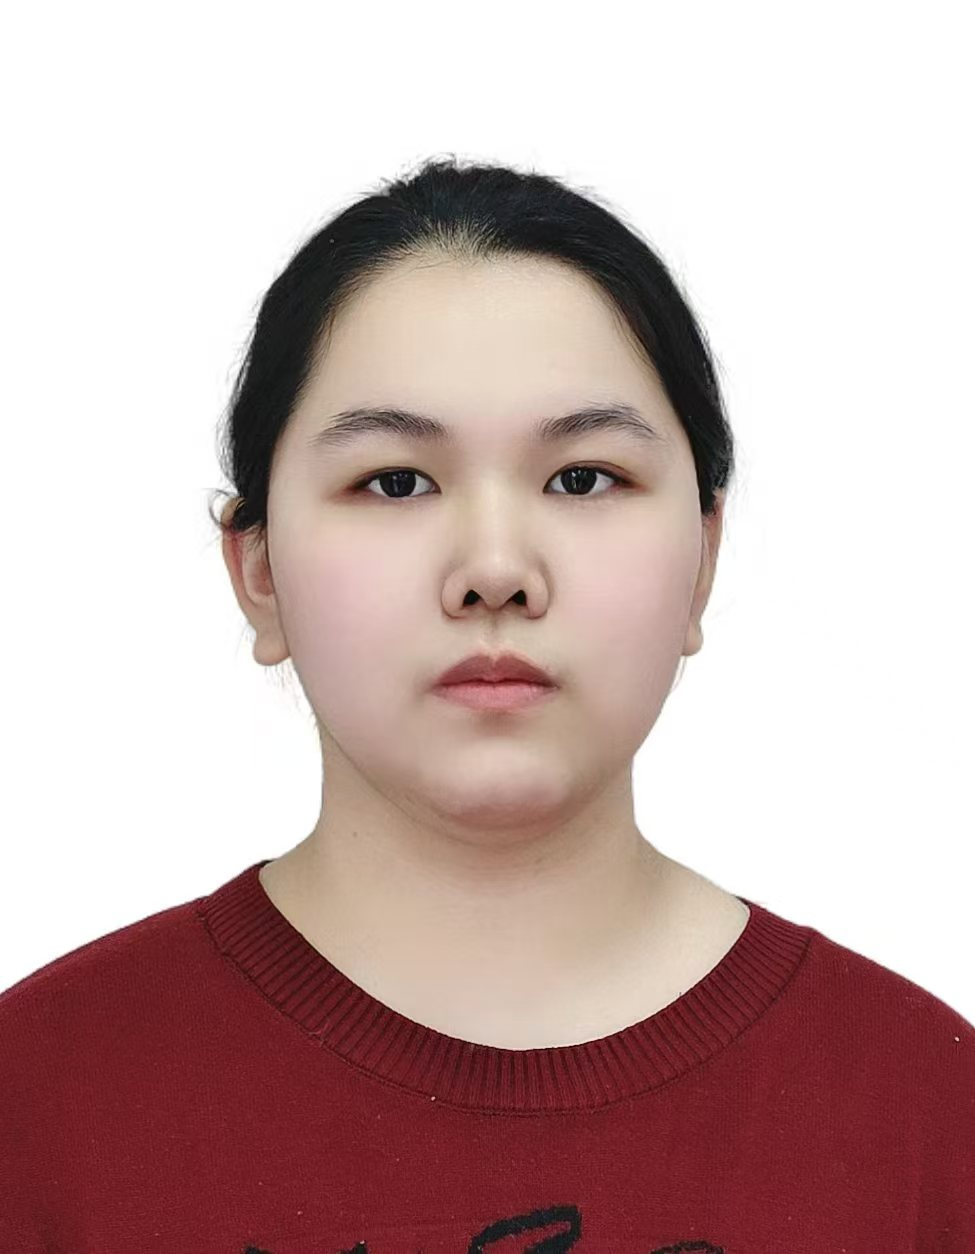
\includegraphics[width=0.8\linewidth,height=\textheight,keepaspectratio]{image/author.jpg}

}

\caption{Фото автора}

\end{figure}%
\end{column}
\end{columns}
\end{frame}

\section{Вводная
часть}\label{ux432ux432ux43eux434ux43dux430ux44f-ux447ux430ux441ux442ux44c}

\begin{frame}{Актуальность и объект}
\protect\phantomsection\label{ux430ux43aux442ux443ux430ux43bux44cux43dux43eux441ux442ux44c-ux438-ux43eux431ux44aux435ux43aux442}
\begin{itemize}
\tightlist
\item
  \textbf{Актуальность:} Навыки установки и настройки Linux --- базовые
  компетенции для любого системного администратора.
\item
  \textbf{Объект исследования:} Процесс установки и первоначальной
  конфигурации ОС.
\item
  \textbf{Предмет исследования:} ОС Rocky Linux 9 и среда виртуализации
  VirtualBox.
\end{itemize}
\end{frame}

\begin{frame}{Научная новизна и значимость}
\protect\phantomsection\label{ux43dux430ux443ux447ux43dux430ux44f-ux43dux43eux432ux438ux437ux43dux430-ux438-ux437ux43dux430ux447ux438ux43cux43eux441ux442ux44c}
\begin{itemize}
\tightlist
\item
  \textbf{Научная новизна:} Освоение современных версий дистрибутивов
  (Rocky Linux 9) и актуальных инструментов виртуализации.
\item
  \textbf{Практическая значимость:} Полученные навыки могут быть
  применены при развертывании серверных инфраструктур и настройке
  рабочих станций.
\end{itemize}
\end{frame}

\begin{frame}[fragile]{Цели и задачи}
\protect\phantomsection\label{ux446ux435ux43bux438-ux438-ux437ux430ux434ux430ux447ux438}
\begin{itemize}
\tightlist
\item
  \textbf{Цель:} Приобретение практических навыков установки ОС на
  виртуальную машину.
\item
  \textbf{Задачи:}

  \begin{itemize}
  \tightlist
  \item
    Создать виртуальную машину в VirtualBox.
  \item
    Установить ОС Rocky Linux 9.
  \item
    Проанализировать последовательность загрузки системы
    (\texttt{dmesg}).
  \item
    Получить информацию о файловых системах.
  \end{itemize}
\end{itemize}
\end{frame}

\begin{frame}[fragile]{Материалы и методы}
\protect\phantomsection\label{ux43cux430ux442ux435ux440ux438ux430ux43bux44b-ux438-ux43cux435ux442ux43eux434ux44b}
\begin{itemize}
\tightlist
\item
  Операционная система: Rocky Linux 9
\item
  Среда виртуализации: Oracle VM VirtualBox
\item
  Основные инструменты: терминал, команды \texttt{dmesg}, \texttt{mount}
\end{itemize}
\end{frame}

\section{Выполнение
работы}\label{ux432ux44bux43fux43eux43bux43dux435ux43dux438ux435-ux440ux430ux431ux43eux442ux44b}

\begin{frame}[fragile]{Создание виртуальной машины}
\protect\phantomsection\label{ux441ux43eux437ux434ux430ux43dux438ux435-ux432ux438ux440ux442ux443ux430ux43bux44cux43dux43eux439-ux43cux430ux448ux438ux43dux44b}
\begin{itemize}
\tightlist
\item
  Создана виртуальная машина \texttt{zhaoxinya}.
\item
  Выделено: 4096 МБ ОЗУ, 2 ядра CPU, 40 ГБ ПЗУ.
\item
  Подключен образ \texttt{Rocky-9.4-x86\_64-dvd.iso}.
\end{itemize}

\begin{figure}[H]

{\centering \pandocbounded{\includegraphics[keepaspectratio]{image/vm_settings.png}}

}

\caption{Параметры ВМ}

\end{figure}%
\end{frame}

\begin{frame}[fragile]{Анализ системы}
\protect\phantomsection\label{ux430ux43dux430ux43bux438ux437-ux441ux438ux441ux442ux435ux43cux44b}
\begin{itemize}
\tightlist
\item
  Проведен анализ журнала \texttt{dmesg}.
\item
  \textbf{Ядро:} 6.12.0-211.16.1.el10\_2.0.1.x86\_64
\item
  \textbf{Процессор:} Intel(R) Core(TM) i9-13900HX (2419.200 MHz)
\item
  \textbf{ОЗУ:} 3.8Gi
\item
  \textbf{Файловая система:} xfs
\end{itemize}

\begin{figure}[H]

{\centering \pandocbounded{\includegraphics[keepaspectratio]{image/dmesg.png}}

}

\caption{Вывод dmesg}

\end{figure}%
\end{frame}

\begin{frame}[fragile]{Монтирование}
\protect\phantomsection\label{ux43cux43eux43dux442ux438ux440ux43eux432ux430ux43dux438ux435}
\begin{itemize}
\tightlist
\item
  Проверена последовательность монтирования через \texttt{mount}.
\item
  Корневой раздел \texttt{/dev/mapper/rl-root} смонтирован как
  \texttt{xfs}.
\end{itemize}

\begin{figure}[H]

{\centering \pandocbounded{\includegraphics[keepaspectratio]{image/mount.png}}

}

\caption{Вывод mount}

\end{figure}%
\end{frame}

\section{Заключение}\label{ux437ux430ux43aux43bux44eux447ux435ux43dux438ux435}

\begin{frame}{Выводы}
\protect\phantomsection\label{ux432ux44bux432ux43eux434ux44b}
\begin{itemize}
\tightlist
\item
  Успешно установлена и сконфигурирована ОС Rocky Linux 9.
\item
  Получены навыки работы с установщиком и командной строкой.
\item
  Проведен анализ загрузки и оборудования.
\item
  \textbf{Все поставленные задачи выполнены в полном объеме.}
\end{itemize}
\end{frame}




\end{document}
